\documentclass[10pt,fleqn]{article} % Default font size and left-justified equations
\usepackage[%
    pdftitle={Modélisation dynamique : cinétique},
    pdfauthor={Xavier Pessoles}]{hyperref}



%%%%%%%%%%%%%%%%%%%%%%%%%%%%%%%%%%%%%%%%%
% Original author:
% Mathias Legrand (legrand.mathias@gmail.com) with modifications by:
% Vel (vel@latextemplates.com)
% License:
% CC BY-NC-SA 3.0 (http://creativecommons.org/licenses/by-nc-sa/3.0/)
%%%%%%%%%%%%%%%%%%%%%%%%%%%%%%%%%%%%%%%%%

%----------------------------------------------------------------------------------------
%	VARIOUS REQUIRED PACKAGES AND CONFIGURATIONS
%----------------------------------------------------------------------------------------

%\usepackage[top=2.5cm,bottom=2cm,left=2cm,right=2cm,headsep=40pt,a4paper]{geometry} % Page margins
\usepackage[top=2cm,bottom=3cm,left=2cm,right=2cm,a4paper]{geometry} % Page margins

\usepackage{graphicx} % Required for including pictures

\usepackage{lipsum} % Inserts dummy text

\usepackage{tikz} % Required for drawing custom shapes

\usepackage[francais]{babel} % English language/hyphenation
\frenchbsetup{StandardLists=true} % Pour éviter la collision babel enumitem pour les listes

\usepackage{enumitem} % Customize lists
\setlist{nolistsep} % Reduce spacing between bullet points and numbered lists

\usepackage{booktabs} % Required for nicer horizontal rules in tables

\usepackage{xcolor} % Required for specifying colors by name
%\definecolor{ocre}{RGB}{243,102,25} % Define the orange color used for highlighting throughout the book
 \definecolor{ocre}{RGB}{49,133,156} % Couleur ''bleue''
\definecolor{violetf}{RGB}{112,48,160} % Couleur ''violet''
\usepackage{enumitem}
\usepackage{pifont} % Pour les dinglist
\usepackage{multicol}
\usepackage{array} % Centrage vertical dans les tableaux
\usepackage{schemabloc}

%----------------------------------------------------------------------------------------
%	FONTS
%----------------------------------------------------------------------------------------
\usepackage{bm}
\usepackage{multicol}
\usepackage{siunitx}
\sisetup{output-decimal-marker = {,}}


\usepackage{avant} % Use the Avantgarde font for headings
%\usepackage{times} % Use the Times font for headings
%\usepackage{mathptmx} % Use the Adobe Times Roman as the default text font together with math symbols from the Sym­bol, Chancery and Com­puter Modern fonts
\usepackage[adobe-utopia]{mathdesign}
\usepackage{microtype} % Slightly tweak font spacing for aesthetics
\usepackage[utf8]{inputenc} % Required for including letters with accents
\usepackage[T1]{fontenc} % Use 8-bit encoding that has 256 glyphs

%----------------------------------------------------------------------------------------
%	BIBLIOGRAPHY AND INDEX
%----------------------------------------------------------------------------------------

%\usepackage[style=alphabetic,citestyle=numeric,sorting=nyt,sortcites=true,autopunct=true,babel=hyphen,hyperref=true,abbreviate=false,backref=true,backend=biber]{biblatex}
\usepackage[style=alphabetic,citestyle=numeric,sorting=nyt,sortcites=true,autopunct=true,hyperref=true,abbreviate=false,backref=true,backend=biber]{biblatex}
\addbibresource{bibliography.bib} % BibTeX bibliography file
\defbibheading{bibempty}{}

\usepackage{calc} % For simpler calculation - used for spacing the index letter headings correctly
\usepackage{makeidx} % Required to make an index
\makeindex % Tells LaTeX to create the files required for indexing

%----------------------------------------------------------------------------------------
%	MAIN TABLE OF CONTENTS
%----------------------------------------------------------------------------------------

\usepackage{titletoc} % Required for manipulating the table of contents

\setcounter{tocdepth}{2}     % Dans la table des matieres
\setcounter{secnumdepth}{2}

\contentsmargin{0cm} % Removes the default margin

% Part text styling
\titlecontents{part}[0cm]
{\addvspace{20pt}\centering\large\bfseries}
{}
{}
{}

% Chapter text styling
\titlecontents{chapter}[1.25cm] % Indentation
{\addvspace{12pt}\large\sffamily\bfseries} % Spacing and font options for chapters
{\color{ocre!60}\contentslabel[\Large\thecontentslabel]{1.25cm}\color{ocre}} % Chapter number
{\color{ocre}}  
{\color{ocre!60}\normalsize\;\titlerule*[.5pc]{.}\;\thecontentspage} % Page number

% Section text styling
\titlecontents{section}[1.25cm] % Indentation
{\addvspace{3pt}\sffamily\bfseries} % Spacing and font options for sections
{\color{ocre!60}\contentslabel[\thecontentslabel]{1.25cm} \color{ocre}} % Section number
{\color{ocre}}
{\hfill\color{ocre!60}\thecontentspage} % Page number
[]

% Subsection text styling
\titlecontents{subsection}[1.25cm] % Indentation
{\addvspace{1pt}\sffamily\small} % Spacing and font options for subsections
{\contentslabel[\thecontentslabel]{1.25cm}} % Subsection number
{}
{\ \titlerule*[.5pc]{.}\;\thecontentspage} % Page number
[]


% Subsection text styling
\titlecontents{subsubsection}[1.25cm] % Indentation
{\addvspace{1pt}\sffamily\small} % Spacing and font options for subsections
{\contentslabel[\thecontentslabel]{1.25cm}} % Subsection number
{}
{\ \titlerule*[.5pc]{.}\;\thecontentspage} % Page number
[]

% List of figures
\titlecontents{figure}[0em]
{\addvspace{-5pt}\sffamily}
{\thecontentslabel\hspace*{1em}}
{}
{\ \titlerule*[.5pc]{.}\;\thecontentspage}
[]

% List of tables
\titlecontents{table}[0em]
{\addvspace{-5pt}\sffamily}
{\thecontentslabel\hspace*{1em}}
{}
{\ \titlerule*[.5pc]{.}\;\thecontentspage}
[]

%----------------------------------------------------------------------------------------
%	MINI TABLE OF CONTENTS IN PART HEADS
%----------------------------------------------------------------------------------------

% Chapter text styling
\titlecontents{lchapter}[0em] % Indenting
{\addvspace{15pt}\large\sffamily\bfseries} % Spacing and font options for chapters
{\color{ocre}\contentslabel[\Large\thecontentslabel]{1.25cm}\color{ocre}} % Chapter number
{}  
{\color{ocre}\normalsize\sffamily\bfseries\;\titlerule*[.5pc]{.}\;\thecontentspage} % Page number

% Section text styling
\titlecontents{lsection}[0em] % Indenting
{\sffamily\small} % Spacing and font options for sections
{\contentslabel[\thecontentslabel]{1.25cm}} % Section number
{}
{}

% Subsection text styling
\titlecontents{lsubsection}[.5em] % Indentation
{\normalfont\footnotesize\sffamily} % Font settings
{}
{}
{}

%----------------------------------------------------------------------------------------
%	PAGE HEADERS
%----------------------------------------------------------------------------------------

\usepackage{fancyhdr} % Required for header and footer configuration



\pagestyle{fancy}
 \renewcommand{\headrulewidth}{0pt}
 \fancyhead{}
 
 % ENTETES de page
 \fancyhead[L]{%
 \noindent\begin{minipage}[c]{2.6cm}%
 
\includegraphics[width=2cm]{logo_lycee.png}%
 \end{minipage}
}

\fancyhead[C]{\rule{8cm}{.5pt}}

 \fancyhead[R]{%
 \noindent\begin{minipage}[c]{3cm}
 \begin{flushright}
 \footnotesize{\textit{\textsf{\xxtete}}}%
 \end{flushright}
 \end{minipage}
}

 \fancyfoot{}
 % PIEDS de page
\fancyfoot[C]{\rule{12cm}{.5pt}}
\renewcommand{\footrulewidth}{0.2pt}
\fancyfoot[C]{\footnotesize{\bfseries \thepage}}
\fancyfoot[L]{ 
\begin{minipage}[c]{.4\linewidth}
\noindent\footnotesize{{\xxauteur}}
\end{minipage}}

\fancyfoot[R]{\footnotesize{\xxpied}
\ifthenelse{\isodd{\value{page}}}{
\begin{tikzpicture}[overlay]
\node[shape=rectangle, 
      rounded corners = .25 cm,
	  draw= ocre,
	  line width=2pt, 
	  fill = ocre!10,
	  minimum width  = 2.5cm,
	  minimum height = 3cm,] at (\xxposongletx,\xxposonglety) {};
\node at (\xxposonglettext,\xxposonglety) {\rotatebox{90}{\textbf{\large\color{ocre}{\xxonglet}}}};
%{};
\end{tikzpicture}}{}
}



%
%
%
% Removes the header from odd empty pages at the end of chapters
\makeatletter
%\renewcommand{\cleardoublepage}{
%\clearpage\ifodd\c@page\else
%\hbox{}
%\vspace*{\fill}
%\thispagestyle{empty}
%\newpage
%\fi}

%\fancypagestyle{plain}{%
%\fancyhf{} % vide l’en-tête et le pied~de~page.
%%\fancyfoot[C]{\bfseries \thepage} % numéro de la page en cours en gras
%% et centré en pied~de~page.
%\fancyfoot[R]{\footnotesize{\xxpied}}
%\fancyfoot[C]{\rule{12cm}{.5pt}}
%\renewcommand{\footrulewidth}{0.2pt}
%\fancyfoot[C]{\footnotesize{\bfseries \thepage}}
%\fancyfoot[L]{ 
%\begin{minipage}[c]{.4\linewidth}
%\noindent\footnotesize{{\xxauteur}}
%\end{minipage}}}

\fancypagestyle{plain}{%
\fancyhf{} % vide l’en-tête et le pied~de~page.
\fancyfoot[C]{\rule{12cm}{.5pt}}
\renewcommand{\footrulewidth}{0.2pt}
\fancyfoot[C]{\footnotesize{\bfseries \thepage}}
\fancyfoot[L]{ 
\begin{minipage}[c]{.4\linewidth}
\noindent\footnotesize{{\xxauteur}}
\end{minipage}}
\fancyfoot[R]{\footnotesize{\xxpied}}
}




%----------------------------------------------------------------------------------------
%	THEOREM STYLES
%----------------------------------------------------------------------------------------

% Conflit avec la police adobe
%\usepackage{amsmath,amsfonts,amssymb,amsthm} % For math equations, theorems, symbols, etc
\usepackage{amsmath,amsthm}

\newcommand{\intoo}[2]{\mathopen{]}#1\,;#2\mathclose{[}}
\newcommand{\ud}{\mathop{\mathrm{{}d}}\mathopen{}}
\newcommand{\intff}[2]{\mathopen{[}#1\,;#2\mathclose{]}}
%\newtheorem{notation}{Notation}[chapter]
\newtheorem{notation}{Notation}[section]

% Boxed/framed environments
\newtheoremstyle{ocrenumbox}% % Theorem style name
{0pt}% Space above
{0pt}% Space below
{\normalfont}% % Body font
{}% Indent amount
{\small\bf\sffamily\color{ocre}}% % Theorem head font
{\;}% Punctuation after theorem head
{0.25em}% Space after theorem head
{\small\sffamily\color{ocre}\thmname{#1}\nobreakspace\thmnumber%{\@ifnotempty{#1}{}\@upn{#2}}% Theorem text (e.g. Theorem 2.1)
\thmnote{\nobreakspace\the\thm@notefont\sffamily\bfseries\color{black}---\nobreakspace#3.}} % Optional theorem note
\renewcommand{\qedsymbol}{$\blacksquare$}% Optional qed square


% Boite pour les corriges
\newtheoremstyle{correctionbox}% % Theorem style name
{0pt}% Space above
{0pt}% Space below
{\normalfont}% % Body font
{}% Indent amount
{\small\bf\sffamily\color{violet}}% % Theorem head font
{\;}% Punctuation after theorem head
{0.25em}% Space after theorem head
{\small\sffamily\color{ocre}\thmname{#1}\nobreakspace\thmnumber%{\@ifnotempty{#1}{}\@upn{#2}}% Theorem text (e.g. Theorem 2.1)
\thmnote{\nobreakspace\the\thm@notefont\sffamily\bfseries\color{black}---\nobreakspace#3.}} % Optional theorem note
\renewcommand{\qedsymbol}{$\blacksquare$}% Optional qed square



\newtheoremstyle{blacknumex}% Theorem style name
{5pt}% Space above
{5pt}% Space below
{\normalfont}% Body font
{} % Indent amount
{\small\bf\sffamily}% Theorem head font
{\;}% Punctuation after theorem head
{0.25em}% Space after theorem head
{\small\sffamily{\tiny\ensuremath{\blacksquare}}\nobreakspace\thmname{#1}\nobreakspace\thmnumber%{\@ifnotempty{#1}{}\@upn{#2}}% Theorem text (e.g. Theorem 2.1)
\thmnote{\nobreakspace\the\thm@notefont\sffamily\bfseries---\nobreakspace#3.}}% Optional theorem note

\newtheoremstyle{blacknumbox} % Theorem style name
{0pt}% Space above
{0pt}% Space below
{\normalfont}% Body font
{}% Indent amount
{\small\bf\sffamily}% Theorem head font
{\;}% Punctuation after theorem head
{0.25em}% Space after theorem head
{\small\sffamily\thmname{#1}\nobreakspace 
\thmnote{\nobreakspace\the\thm@notefont\sffamily\bfseries---\nobreakspace#3.}}% Optional theorem note

% Non-boxed/non-framed environments
\newtheoremstyle{ocrenum}% % Theorem style name
{5pt}% Space above
{5pt}% Space below
{\normalfont}% % Body font
{}% Indent amount
{\small\bf\sffamily\color{ocre}}% % Theorem head font
{\;}% Punctuation after theorem head
{0.25em}% Space after theorem head
{\small\sffamily\color{ocre}\thmname{#1}\nobreakspace%\thmnumber{\@ifnotempty{#1}{}\@upn{#2}}% Theorem text (e.g. Theorem 2.1)
\thmnote{\nobreakspace\the\thm@notefont\sffamily\bfseries\color{black}---\nobreakspace#3.}} % Optional theorem note
\renewcommand{\qedsymbol}{$\blacksquare$}% Optional qed square
\makeatother

% Environnement pour les titres de parties
\newtheoremstyle{partiebox} 
{0pt}% Space above
{0pt}% Space below
{\normalfont}% Body font
{}% Indent amount
{\small\bf\sffamily}% Theorem head font
{\;}% Punctuation after theorem head
{0.25em}% Space after theorem head




% Defines the theorem text style for each type of theorem to one of the three styles above
\newcounter{dummy} 
\numberwithin{dummy}{section}
\theoremstyle{ocrenumbox}
%\newtheorem{theoremeT}[dummy]{Théorème}
\newtheorem{theoremeT}[dummy]{Théorème}
\newtheorem{resultatT}[dummy]{Résultat}
\newtheorem{savoirT}[dummy]{Savoir}
\newtheorem{methodeT}[dummy]{Méthode}
\newtheorem{objectifT}[dummy]{Objectif}
%\newtheorem{problem}{Problem}[chapter]
\newtheorem{problem}{Problem}[section]
%\newtheorem{exerciseT}{Exercise}[chapter]
\newtheorem{exerciseT}{Exercice}[section]

\theoremstyle{blacknumex}
%\newtheorem{exampleT}{Example}[chapter]
\newtheorem{exempleT}{Exemple}[section]
\newtheorem{termT}{Terminal\\}[section]
\newtheorem{pyT}{Python\\}[section]
\newtheorem{sciT}{Scilab\\}[section]
\newtheorem{pseudoT}{Pseudo Code\\}[section]
\newtheorem{sqlT}{SQL\\}[section]

\theoremstyle{blacknumbox}
%\newtheorem{vocabulary}{Vocabulary}[chapter]
\newtheorem{vocabulary}{Vocabulaire}[section]
%\newtheorem{definitionT}{Definition}[section]
\newtheorem{definitionT}{Définition}[section]
\newtheorem{rappelT}{Rappel}[section]
\newtheorem{demoT}{Démonstration}[section]
\newtheorem{corollaryT}[dummy]{Corollaire}
\newtheorem{hypoT}{Hypothèse(s)}

\theoremstyle{ocrenum}
\newtheorem{proposition}[dummy]{Proposition}

\theoremstyle{partiebox}
\newtheorem{titrepartieT}[]{}
\newtheorem{titrechapitreT}[]{}

\theoremstyle{correctionbox}
\newtheorem{correctionT}[dummy]{\color{violet}{Correction}}

%----------------------------------------------------------------------------------------
%	DEFINITION OF COLORED BOXES
%----------------------------------------------------------------------------------------

\RequirePackage[framemethod=tikz]{mdframed} % Required for creating the theorem, definition, exercise and corollary boxes

% Theorem box
\newmdenv[skipabove=7pt,
skipbelow=7pt,
backgroundcolor=ocre!10,
linecolor=ocre,
innerleftmargin=5pt,
innerrightmargin=5pt,
innertopmargin=5pt,
leftmargin=0cm,
rightmargin=0cm,
innerbottommargin=5pt]{tBox}


% Correction
\newmdenv[skipabove=7pt,
skipbelow=7pt,
backgroundcolor=violet!10,
linecolor=violet,
innerleftmargin=5pt,
innerrightmargin=5pt,
innertopmargin=5pt,
leftmargin=0cm,
rightmargin=0cm,
innerbottommargin=5pt]{coBox}


% Exercise box	  
\newmdenv[skipabove=7pt,
skipbelow=7pt,
rightline=false,
leftline=true,
topline=false,
bottomline=false,
backgroundcolor=ocre!10,
linecolor=ocre,
innerleftmargin=5pt,
innerrightmargin=5pt,
innertopmargin=5pt,
innerbottommargin=5pt,
leftmargin=0cm,
rightmargin=0cm,
linewidth=4pt]{eBox}	

% Definition box
\newmdenv[skipabove=7pt,
skipbelow=7pt,
rightline=false,
leftline=true,
topline=false,
bottomline=false,
backgroundcolor=ocre!10,
linecolor=ocre,
innerleftmargin=5pt,
innerrightmargin=5pt,
innertopmargin=0pt,
leftmargin=0cm,
rightmargin=0cm,
linewidth=4pt,
innerbottommargin=0pt]{dBox}	

% Demonstration box
\newmdenv[skipabove=7pt,
skipbelow=7pt,
rightline=false,
leftline=true,
topline=false,
bottomline=false,
%backgroundcolor=ocre!10,
linecolor=ocre,
innerleftmargin=5pt,
innerrightmargin=5pt,
innertopmargin=0pt,
leftmargin=0cm,
rightmargin=0cm,
linewidth=4pt,
innerbottommargin=0pt]{demoBox}	

% Corollary box
\newmdenv[skipabove=7pt,
skipbelow=7pt,
rightline=false,
leftline=true,
topline=false,
bottomline=false,
linecolor=gray,
backgroundcolor=black!5,
innerleftmargin=5pt,
innerrightmargin=5pt,
innertopmargin=5pt,
leftmargin=0cm,
rightmargin=0cm,
linewidth=4pt,
innerbottommargin=5pt]{cBox}


% Hypothèses
\newmdenv[skipabove=7pt,
skipbelow=7pt,
rightline=false,
leftline=true,
topline=false,
bottomline=false,
linecolor=gray,
backgroundcolor=black!5,
innerleftmargin=5pt,
innerrightmargin=5pt,
innertopmargin=5pt,
leftmargin=0cm,
rightmargin=0cm,
linewidth=4pt,
innerbottommargin=5pt]{hyBox}


% Boite pour le titre de la partie (pBox)
\newmdenv[skipabove=7pt,
skipbelow=7pt,
rightline=true,
leftline=false,
topline=false,
bottomline=false,
linecolor=ocre,
backgroundcolor=none,
innerleftmargin=5pt,
innerrightmargin=5pt,
innertopmargin=5pt,
leftmargin=0cm,
rightmargin=0cm,
linewidth=4pt,
innerbottommargin=5pt]{pBox}

% Boite pour le titre du chapitre (chBox)
\newmdenv[skipabove=7pt,
skipbelow=7pt,
rightline=false,
leftline=true,
topline=false,
bottomline=false,
linecolor=ocre,
%backgroundcolor=black!5,
innerleftmargin=5pt,
innerrightmargin=5pt,
innertopmargin=5pt,
leftmargin=0cm,
rightmargin=0cm,
linewidth=4pt,
innerbottommargin=5pt]{chBox}


% Boite pour les exemples
\newmdenv[skipabove=7pt,
skipbelow=7pt,
rightline=false,
leftline=true,
topline=false,
bottomline=false,
linecolor=gray,
backgroundcolor=white,
innerleftmargin=5pt,
innerrightmargin=5pt,
innertopmargin=5pt,
leftmargin=0cm,
rightmargin=0cm,
linewidth=4pt,
innerbottommargin=5pt]{exBox}

% Boite pour le terminal
\newmdenv[skipabove=7pt,
skipbelow=7pt,
rightline=false,
leftline=true,
topline=false,
bottomline=false,
linecolor=gray,
backgroundcolor=white,
innerleftmargin=5pt,
innerrightmargin=5pt,
innertopmargin=5pt,
leftmargin=0cm,
rightmargin=0cm,
linewidth=4pt,
innerbottommargin=5pt]{termBox}


% Boite pour Python
\newmdenv[skipabove=7pt,
skipbelow=7pt,
rightline=false,
leftline=true,
topline=false,
bottomline=false,
linecolor=gray,
backgroundcolor=white,
innerleftmargin=5pt,
innerrightmargin=5pt,
innertopmargin=0pt,
leftmargin=0cm,
rightmargin=0cm,
linewidth=4pt,
innerbottommargin=5pt]{pyBox}

% Boite pour scilab
\newmdenv[skipabove=7pt,
skipbelow=7pt,
rightline=false,
leftline=true,
topline=false,
bottomline=false,
linecolor=gray,
backgroundcolor=white,
innerleftmargin=5pt,
innerrightmargin=5pt,
innertopmargin=5pt,
leftmargin=0cm,
rightmargin=0cm,
linewidth=4pt,
innerbottommargin=5pt]{sciBox}


% Boite pour pseudo
\newmdenv[skipabove=7pt,
skipbelow=7pt,
rightline=false,
leftline=true,
topline=false,
bottomline=false,
linecolor=gray,
backgroundcolor=white,
innerleftmargin=5pt,
innerrightmargin=5pt,
innertopmargin=5pt,
leftmargin=0cm,
rightmargin=0cm,
linewidth=4pt,
innerbottommargin=5pt]{pseudoBox}

% Boite pour pseudo
\newmdenv[skipabove=7pt,
skipbelow=7pt,
rightline=false,
leftline=true,
topline=false,
bottomline=false,
linecolor=gray,
backgroundcolor=white,
innerleftmargin=5pt,
innerrightmargin=5pt,
innertopmargin=5pt,
leftmargin=0cm,
rightmargin=0cm,
linewidth=4pt,
innerbottommargin=5pt]{sqlBox}


% Creates an environment for each type of theorem and assigns it a theorem text style from the "Theorem Styles" section above and a colored box from above
\newenvironment{theorem}{\begin{tBox}\begin{theoremeT}}{\end{theoremeT}\end{tBox}}
\newenvironment{resultat}{\begin{tBox}\begin{resultatT}}{\end{resultatT}\end{tBox}}
\newenvironment{methode}{\begin{tBox}\begin{methodeT}}{\end{methodeT}\end{tBox}}
\newenvironment{savoir}{\begin{tBox}\begin{savoirT}}{\end{savoirT}\end{tBox}}
\newenvironment{obj}{\begin{tBox}\begin{objectifT}}{\end{objectifT}\end{tBox}}
\newenvironment{corrige}{\begin{coBox}\begin{correctionT}}{\end{correctionT}\end{coBox}}
\newenvironment{exercise}{\begin{eBox}\begin{exerciseT}}{\hfill{\color{ocre}\tiny\ensuremath{\blacksquare}}\end{exerciseT}\end{eBox}}				  
\newenvironment{exercice}{\begin{eBox}\begin{exerciseT}}{\hfill{\color{ocre}\tiny\ensuremath{\blacksquare}}\end{exerciseT}\end{eBox}}				  

\newenvironment{definition}{\begin{dBox}\begin{definitionT}}{\end{definitionT}\end{dBox}}	
\newenvironment{rappel}{\begin{dBox}\begin{rappelT}}{\end{rappelT}\end{dBox}}	
\newenvironment{defi}{\begin{dBox}\begin{definitionT}}{\end{definitionT}\end{dBox}}	
\newenvironment{demo}{\begin{demoBox}\begin{demoT}}{\end{demoT}\end{demoBox}}	
%\newenvironment{exemple}{\begin{exempleT}}{\hfill{\tiny\ensuremath{\blacksquare}}\end{exempleT}}		
\newenvironment{corollary}{\begin{cBox}\begin{corollaryT}}{\end{corollaryT}\end{cBox}}
\newenvironment{hypo}{\begin{hyBox}\begin{hypoT}}{\end{hypoT}\end{hyBox}}	\newenvironment{exemple}{\begin{exBox}\begin{exempleT}}{\hfill{\tiny\ensuremath{\blacksquare}}\end{exempleT}\end{exBox}}	
\newenvironment{titrepartie}{\begin{pBox}\begin{titrepartieT}}{\end{titrepartieT}\end{pBox}}	
\newenvironment{titrechapitre}{\begin{chBox}\begin{titrechapitreT}}{\end{titrechapitreT}\end{chBox}}	

\newenvironment{term}{ \begin{termBox}\begin{termT}}{\end{termT}\end{termBox}}
\newenvironment{py}{ \begin{pyBox}\begin{pyT}}{\end{pyT}\end{pyBox}}
\newenvironment{sci}{ \begin{sciBox}\begin{sciT}}{\end{sciT}\end{sciBox}}
\newenvironment{pseudo}{ \begin{pseudoBox}\begin{pseudoT}}{\end{pseudoT}\end{pseudoBox}}
\newenvironment{envsql}{ \begin{sqlBox}\begin{sqlT}}{\end{sqlT}\end{sqlBox}}


%----------------------------------------------------------------------------------------
%	REMARK ENVIRONMENT
%----------------------------------------------------------------------------------------

\newenvironment{remark}{\par\vspace{10pt}\small % Vertical white space above the remark and smaller font size
\begin{list}{}{
\leftmargin=35pt % Indentation on the left
\rightmargin=25pt}\item\ignorespaces % Indentation on the right
\makebox[-2.5pt]{\begin{tikzpicture}[overlay]
\node[draw=ocre!60,line width=1pt,circle,fill=ocre!25,font=\sffamily\bfseries,inner sep=2pt,outer sep=0pt] at (-15pt,0pt){\textcolor{ocre}{R}};\end{tikzpicture}} % Orange R in a circle
\advance\baselineskip -1pt}{\end{list}\vskip5pt} % Tighter line spacing and white space after remark

\newenvironment{rem}{\par\vspace{10pt}\small % Vertical white space above the remark and smaller font size
\begin{list}{}{
\leftmargin=35pt % Indentation on the left
\rightmargin=25pt}\item\ignorespaces % Indentation on the right
\makebox[-2.5pt]{\begin{tikzpicture}[overlay]
\node[draw=ocre!60,line width=1pt,circle,fill=ocre!25,font=\sffamily\bfseries,inner sep=2pt,outer sep=0pt] at (-15pt,0pt){\textcolor{ocre}{R}};\end{tikzpicture}} % Orange R in a circle
\advance\baselineskip -1pt}{\end{list}\vskip5pt} % Tighter line spacing and white space after remark


\newenvironment{warn}{\par\vspace{10pt}\small % Vertical white space above the remark and smaller font size
\begin{list}{}{
\leftmargin=35pt % Indentation on the left
\rightmargin=25pt}\item\ignorespaces % Indentation on the right
\makebox[-2.5pt]{\begin{tikzpicture}[overlay]
\node[draw=red!60,line width=1pt,circle,fill=red!25,font=\sffamily\bfseries,inner sep=2pt,outer sep=0pt] at (-15pt,0pt){\textcolor{black}{!}};\end{tikzpicture}} % Point d'exclamation dans un cercle
\advance\baselineskip -1pt}{\end{list}\vskip5pt} % Tighter line spacing and white space after remark


%----------------------------------------------------------------------------------------
%	SECTION NUMBERING IN THE MARGIN
%----------------------------------------------------------------------------------------
\setcounter{secnumdepth}{3}
\setcounter{tocdepth}{2}



\makeatletter
\renewcommand{\@seccntformat}[1]{\llap{\textcolor{ocre}{\csname the#1\endcsname}\hspace{1em}}}                    
\renewcommand{\section}{\@startsection{section}{1}{\z@}
{-4ex \@plus -1ex \@minus -.4ex}
{1ex \@plus.2ex }
{\normalfont\large\sffamily\bfseries}}
\renewcommand{\subsection}{\@startsection {subsection}{2}{\z@}
{-3ex \@plus -0.1ex \@minus -.4ex}
{0.5ex \@plus.2ex }
{\normalfont\sffamily\bfseries}}
\renewcommand{\subsubsection}{\@startsection {subsubsection}{3}{\z@}
{-2ex \@plus -0.1ex \@minus -.2ex}
{.2ex \@plus.2ex }
{\normalfont\small\sffamily\bfseries}}                        
\renewcommand\paragraph{\@startsection{paragraph}{4}{\z@}
{-2ex \@plus-.2ex \@minus .2ex}
{.1ex}
{\normalfont\small\sffamily\bfseries}}

%----------------------------------------------------------------------------------------
%	PART HEADINGS
%----------------------------------------------------------------------------------------


%----------------------------------------------------------------------------------------
%	CHAPTER HEADINGS
%----------------------------------------------------------------------------------------

% \newcommand{\thechapterimage}{}%
% \newcommand{\chapterimage}[1]{\renewcommand{\thechapterimage}{#1}}%
% \def\@makechapterhead#1{%
% {\parindent \z@ \raggedright \normalfont
% \ifnum \c@secnumdepth >\m@ne
% \if@mainmatter
% \begin{tikzpicture}[remember picture,overlay]
% \node at (current page.north west)
% {\begin{tikzpicture}[remember picture,overlay]
% \node[anchor=north west,inner sep=0pt] at (0,0) {\includegraphics[width=\paperwidth]{\thechapterimage}};
% \draw[anchor=west] (\Gm@lmargin,-9cm) node [line width=2pt,rounded corners=15pt,draw=ocre,fill=white,fill opacity=0.5,inner sep=15pt]{\strut\makebox[22cm]{}};
% \draw[anchor=west] (\Gm@lmargin+.3cm,-9cm) node {\huge\sffamily\bfseries\color{black}\thechapter. #1\strut};
% \end{tikzpicture}};
% \end{tikzpicture}
% \else
% \begin{tikzpicture}[remember picture,overlay]
% \node at (current page.north west)
% {\begin{tikzpicture}[remember picture,overlay]
% \node[anchor=north west,inner sep=0pt] at (0,0) {\includegraphics[width=\paperwidth]{\thechapterimage}};
% \draw[anchor=west] (\Gm@lmargin,-9cm) node [line width=2pt,rounded corners=15pt,draw=ocre,fill=white,fill opacity=0.5,inner sep=15pt]{\strut\makebox[22cm]{}};
% \draw[anchor=west] (\Gm@lmargin+.3cm,-9cm) node {\huge\sffamily\bfseries\color{black}#1\strut};
% \end{tikzpicture}};
% \end{tikzpicture}
% \fi\fi\par\vspace*{270\p@}}}

%-------------------------------------------

\def\@makeschapterhead#1{%
\begin{tikzpicture}[remember picture,overlay]
\node at (current page.north west)
{\begin{tikzpicture}[remember picture,overlay]
\node[anchor=north west,inner sep=0pt] at (0,0) {\includegraphics[width=\paperwidth]{\thechapterimage}};
\draw[anchor=west] (\Gm@lmargin,-9cm) node [line width=2pt,rounded corners=15pt,draw=ocre,fill=white,fill opacity=0.5,inner sep=15pt]{\strut\makebox[22cm]{}};
\draw[anchor=west] (\Gm@lmargin+.3cm,-9cm) node {\huge\sffamily\bfseries\color{black}#1\strut};
\end{tikzpicture}};
\end{tikzpicture}
\par\vspace*{270\p@}}
\makeatother

%----------------------------------------------------------------------------------------
%	HYPERLINKS IN THE DOCUMENTS
%----------------------------------------------------------------------------------------


\hypersetup{hidelinks,backref=true,pagebackref=true,hyperindex=true,colorlinks=false,breaklinks=true,urlcolor= ocre,bookmarks=true,bookmarksopen=false,pdftitle={Title},pdfauthor={Author}}
\usepackage{bookmark}
\bookmarksetup{
open,
numbered,
addtohook={%
\ifnum\bookmarkget{level}=0 % chapter
\bookmarksetup{bold}%
\fi
\ifnum\bookmarkget{level}=-1 % part
\bookmarksetup{color=ocre,bold}%
\fi
}
}

%----------------------------------------------------------------------------------------
%	
%----------------------------------------------------------------------------------------

\newcommand{\thechapterimage}{}%
\newcommand{\chapterimage}[1]{\renewcommand{\thechapterimage}{#1}}%
\def\@makechapterhead#1{%
{\parindent \z@ \raggedright \normalfont
\begin{tikzpicture}[remember picture,overlay]
\node at (current page.north west)
{\begin{tikzpicture}[remember picture,overlay]
\node[anchor=north west,inner sep=0pt] at (0,0) {\includegraphics[width=\paperwidth]{\thechapterimage}};
%\draw[anchor=west] (\Gm@lmargin,-9cm) node [line width=2pt,rounded corners=15pt,draw=ocre,fill=white,fill opacity=0.5,inner sep=15pt]{\strut\makebox[22cm]{}};
%\draw[anchor=west] (\Gm@lmargin+.3cm,-9cm) node {\huge\sffamily\bfseries\color{black}\thechapter. #1\strut};
\end{tikzpicture}};
\end{tikzpicture}
\par\vspace*{270\p@}
}}

 \newcounter{exo}


\makeatletter             
\renewcommand{\subparagraph}{\@startsection{exo}{5}{\z@}%
                                    {-2ex \@plus-.2ex \@minus .2ex}%
                                    {0ex}%               
{\normalfont\bfseries Question \hspace{.7cm} }}
\makeatother
\renewcommand{\thesubparagraph}{\arabic{subparagraph}} 
\makeatletter


\usepackage{textcomp}

% Définition des booleéns
\newif\iffiche
\newif\ifprof
\newif\iftd
\newif\ifcours
\newif\ifnormal
\newif\ifdifficile
\newif\iftdifficile
\newif\ifcolle
\newif\iflivret
%%%%%%%%%%%%
% Définition des vecteurs 
%%%%%%%%%%%%
\newcommand{\vect}[1]{\overrightarrow{#1}}
\newcommand{\axe}[2]{\left(#1,\vect{#2}\right)}
\newcommand{\couple}[2]{\left(#1,\vect{#2}\right)}
\newcommand{\angl}[2]{\left(\vect{#1},\vect{#2}\right)}

\newcommand{\rep}[1]{\mathcal{R}_{#1}}
\newcommand{\quadruplet}[4]{\left(#1;#2,#3,#4 \right)}
\newcommand{\repere}[4]{\left(#1;\vect{#2},\vect{#3},\vect{#4} \right)}
\newcommand{\base}[3]{\left(\vect{#1},\vect{#2},\vect{#3} \right)}


\newcommand{\vx}[1]{\vect{x_{#1}}}
\newcommand{\vy}[1]{\vect{y_{#1}}}
\newcommand{\vz}[1]{\vect{z_{#1}}}

% d droit pour le calcul différentiel
\newcommand{\dd}{\text{d}}

\newcommand{\inertie}[2]{I_{#1}\left( #2\right)}
\newcommand{\matinertie}[7]{
\begin{pmatrix}
#1 & #6 & #5 \\
#6 & #2 & #4 \\
#5 & #4 & #3 \\
\end{pmatrix}_{#7}}
%%%%%%%%%%%%
% Définition des torseurs 
%%%%%%%%%%%%

\newcommand{\ec}[2]{%
\mathcal{E}_c\left(#1/#2\right)}

\newcommand{\pext}[3]{%
\mathcal{P}\left(#1\rightarrow#2/#3\right)}

\newcommand{\pint}[3]{%
\mathcal{P}\left(#1 \stackrel{\text{#3}}{\leftrightarrow} #2\right)}


 \newcommand{\torseur}[1]{%
\left\{{#1}\right\}
}

\newcommand{\torseurcin}[3]{%
\left\{\mathcal{#1} \left(#2/#3 \right) \right\}
}

\newcommand{\torseurci}[2]{%
\left\{\sigma \left(#1/#2 \right) \right\}
}
\newcommand{\torseurdyn}[2]{%
\left\{\mathcal{D} \left(#1/#2 \right) \right\}
}


\newcommand{\torseurstat}[3]{%
\left\{\mathcal{#1} \left(#2\rightarrow #3 \right) \right\}
}


 \newcommand{\torseurc}[8]{%
%\left\{#1 \right\}=
\left\{
{#1}
\right\}
 = 
\left\{%
\begin{array}{cc}%
{#2} & {#5}\\%
{#3} & {#6}\\%
{#4} & {#7}\\%
\end{array}%
\right\}_{#8}%
}

 \newcommand{\torseurcol}[7]{
\left\{%
\begin{array}{cc}%
{#1} & {#4}\\%
{#2} & {#5}\\%
{#3} & {#6}\\%
\end{array}%
\right\}_{#7}%
}

 \newcommand{\torseurl}[3]{%
%\left\{\mathcal{#1}\right\}_{#2}=%
\left\{%
\begin{array}{l}%
{#1} \\%
{#2} %
\end{array}%
\right\}_{#3}%
}

% Vecteur vitesse
 \newcommand{\vectv}[3]{%
\vect{V\left( {#1} \in {#2}/{#3}\right)}
}

% Vecteur force
\newcommand{\vectf}[2]{%
\vect{R\left( {#1} \rightarrow {#2}\right)}
}

% Vecteur moment stat
\newcommand{\vectm}[3]{%
\vect{\mathcal{M}\left( {#1}, {#2} \rightarrow {#3}\right)}
}




% Vecteur résultante cin
\newcommand{\vectrc}[2]{%
\vect{R_c \left( {#1}/ {#2}\right)}
}
% Vecteur moment cin
\newcommand{\vectmc}[3]{%
\vect{\sigma \left( {#1}, {#2} /{#3}\right)}
}


% Vecteur résultante dyn
\newcommand{\vectrd}[2]{%
\vect{R_d \left( {#1}/ {#2}\right)}
}
% Vecteur moment dyn
\newcommand{\vectmd}[3]{%
\vect{\delta \left( {#1}, {#2} /{#3}\right)}
}

% Vecteur accélération
 \newcommand{\vectg}[3]{%
\vect{\Gamma \left( {#1} \in {#2}/{#3}\right)}
}

% Vecteur omega
 \newcommand{\vecto}[2]{%
\vect{\Omega\left( {#1}/{#2}\right)}
}
% }$$\left\{\mathcal{#1} \right\}_{#2} =%
% \left\{%
% \begin{array}{c}%
%  #3 \\%
%  #4 %
% \end{array}%
% \right\}_{#5}}
\usepackage{multicol}
\usepackage{siunitx}

\fichetrue
%\fichefalse

\proftrue
%\proffalse

\tdtrue
%\tdfalse

\courstrue
\coursfalse


\def\discipline{Sciences \\Industrielles de \\ l'Ingénieur}
\def\xxtete{Sciences Industrielles de l'Ingénieur}

\def\classe{\textsf{PSI$\star$ -- MP}}
\def\xxnumpartie{Cycle 04}
\def\xxpartie{Modéliser le comportement des systèmes mécaniques dans le but d'établir une loi de comportement ou de déterminer des actions mécaniques en utilisant le PFD}

\def\xxnumchapitre{Chapitre 3 \vspace{.2cm}}
\def\xxchapitre{\hspace{.12cm} Application du Principe Fondamental de la Dynamique}





\def\xxactivite{Activation 01}
\def\xxauteur{\textsl{Xavier Pessoles}}


\def\xxtitreexo{Assistance pour le maniement de charges dans l’industrie}
\def\xxsourceexo{\hspace{.2cm} \footnotesize{Concours Centrale Supelec TSI 2017}}




  
\def\xxposongletx{2}
\def\xxposonglettext{1.45}
\def\xxposonglety{20}
%\def\xxonglet{Part. 1 -- Ch. 3}
\def\xxonglet{\textsf{Cycle 04}}

\def\xxactivite{Activation 01}
\def\xxauteur{\textsl{Xavier Pessoles}}

\def\xxcompetences{%
\vspace{-.5cm}
\textsl{%
\textbf{Savoirs et compétences :}
\begin{itemize}[label=\ding{112},font=\color{ocre}] 
%\item \textit{Mod2.C16} : torseur cinétique
%\item \textit{Mod2.C17} : torseur dynamique
\item \textit{Mod2.C17.SF1} : déterminer le torseur dynamique d’un solide, ou d’un ensemble de solides, par rapport à un autre solide
%\item \textit{Mod2.C15} : matrice d'inertie
\item \textit{Res1.C2} : principe fondamental de la dynamique
%\item \textit{Res1.C1.SF1} : proposer une démarche permettant la détermination de la loi de mouvement
%\item \textit{Res1.C2.SF1} : proposer une méthode permettant la détermination d’une inconnue de liaison
\end{itemize}
}}
\def\xxfigures{
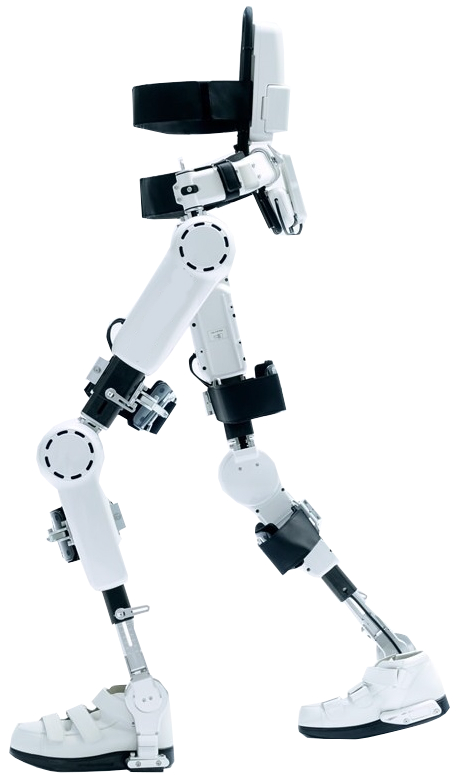
\includegraphics[width=.3\linewidth]{images/fig_01}}%figues de la page de garde


\def\xxpied{%
Cycle 04 -- Modélisation mécanique -- PFD\\% afin de valider leurs performances.\\
Chapitre 3 -- \xxactivite%
}

\setcounter{secnumdepth}{5}
%---------------------------------------------------------------------------


\begin{document}
%\chapterimage{png/Fond_Cin}
\pagestyle{empty}


%%%%%%%% PAGE DE GARDE COURS
\ifcours
% ==== BANDEAU DES TITRES ==== 
\begin{tikzpicture}[remember picture,overlay]
\node at (current page.north west)
{\begin{tikzpicture}[remember picture,overlay]
\node[anchor=north west,inner sep=0pt] at (0,0) {\includegraphics[width=\paperwidth]{\thechapterimage}};
\draw[anchor=west] (-2cm,-8cm) node [line width=2pt,rounded corners=15pt,draw=ocre,fill=white,fill opacity=0.6,inner sep=40pt]{\strut\makebox[22cm]{}};
\draw[anchor=west] (1cm,-8cm) node {\huge\sffamily\bfseries\color{black} %
\begin{minipage}{1cm}
\rotatebox{90}{\LARGE\sffamily\textsc{\color{ocre}\textbf{\xxnumpartie}}}
\end{minipage} \hfill
\begin{minipage}[c]{14cm}
\begin{titrepartie}
\begin{flushright}
\renewcommand{\baselinestretch}{1.1} 
\Large\sffamily\textsc{\textbf{\xxpartie}}
\renewcommand{\baselinestretch}{1} 
\end{flushright}
\end{titrepartie}
\end{minipage} \hfill
\begin{minipage}[c]{3.5cm}
{\large\sffamily\textsc{\textbf{\color{ocre} \discipline}}}
\end{minipage} 
 };
\end{tikzpicture}};
\end{tikzpicture}
% ==== FIN BANDEAU DES TITRES ==== 


% ==== ONGLET 
\begin{tikzpicture}[overlay]
\node[shape=rectangle, 
      rounded corners = .25 cm,
	  draw= ocre,
	  line width=2pt, 
	  fill = ocre!10,
	  minimum width  = 2.5cm,
	  minimum height = 3cm,] at (18.3cm,0) {};
\node at (17.7cm,0) {\rotatebox{90}{\textbf{\Large\color{ocre}{\classe}}}};
%{};
\end{tikzpicture}
% ==== FIN ONGLET 


\vspace{3.5cm}

\begin{tikzpicture}[remember picture,overlay]
\draw[anchor=west] (-2cm,-6cm) node {\huge\sffamily\bfseries\color{black} %
\begin{minipage}{2cm}
\begin{center}
\LARGE\sffamily\textsc{\color{ocre}\textbf{\xxactivite}}
\end{center}
\end{minipage} \hfill
\begin{minipage}[c]{15cm}
\begin{titrechapitre}
\renewcommand{\baselinestretch}{1.1} 
\Large\sffamily\textsc{\textbf{\xxnumchapitre}}

\Large\sffamily\textsc{\textbf{\xxchapitre}}
\vspace{.5cm}

\renewcommand{\baselinestretch}{1} 
\normalsize\normalfont
\xxcompetences
\end{titrechapitre}
\end{minipage}  };
\end{tikzpicture}
\vfill

\begin{flushright}
\begin{minipage}[c]{.3\linewidth}
\begin{center}
\xxfigures
\end{center}
\end{minipage}\hfill
\begin{minipage}[c]{.6\linewidth}
\startcontents
%\printcontents{}{1}{}
\printcontents{}{1}{}
\end{minipage}
\end{flushright}

\begin{tikzpicture}[remember picture,overlay]
\draw[anchor=west] (4.5cm,-.7cm) node {
\begin{minipage}[c]{.2\linewidth}
\begin{flushright}

\includegraphics[width=2cm]{logoCC}
\end{flushright}
\end{minipage}
\begin{minipage}[c]{.2\linewidth}
\textsl{\xxauteur} \\
\textsl{\classe}
\end{minipage}
 };
\end{tikzpicture}

\newpage
\pagestyle{fancy}

%\newpage
%\pagestyle{fancy}

\else
\fi
%% FIN PAGE DE GARDE DES COURS

%%%%%%%% PAGE DE GARDE TD
\iftd
%\begin{tikzpicture}[remember picture,overlay]
%\node at (current page.north west)
%{\begin{tikzpicture}[remember picture,overlay]
%\draw[anchor=west] (-2cm,-3.25cm) node [line width=2pt,rounded corners=15pt,draw=ocre,fill=white,fill opacity=0.6,inner sep=40pt]{\strut\makebox[22cm]{}};
%\draw[anchor=west] (1cm,-3.25cm) node {\huge\sffamily\bfseries\color{black} %
%\begin{minipage}{1cm}
%\rotatebox{90}{\LARGE\sffamily\textsc{\color{ocre}\textbf{\xxnumpartie}}}
%\end{minipage} \hfill
%\begin{minipage}[c]{13.5cm}
%\begin{titrepartie}
%\begin{flushright}
%\renewcommand{\baselinestretch}{1.1} 
%\Large\sffamily\textsc{\textbf{\xxpartie}}
%\renewcommand{\baselinestretch}{1} 
%\end{flushright}
%\end{titrepartie}
%\end{minipage} \hfill
%\begin{minipage}[c]{3.5cm}
%{\large\sffamily\textsc{\textbf{\color{ocre} \discipline}}}
%\end{minipage} 
% };
%\end{tikzpicture}};
%\end{tikzpicture}

%%%%%%%%%% PAGE DE GARDE TD %%%%%%%%%%%%%%%
%\begin{tikzpicture}[overlay]
%\node[shape=rectangle, 
%      rounded corners = .25 cm,
%	  draw= ocre,
%	  line width=2pt, 
%	  fill = ocre!10,
%	  minimum width  = 2.5cm,
%	  minimum height = 2.5cm,] at (18.5cm,0) {};
%\node at (17.7cm,0) {\rotatebox{90}{\textbf{\Large\color{ocre}{\classe}}}};
%%{};
%\end{tikzpicture}

% PARTIE ET CHAPITRE
%\begin{tikzpicture}[remember picture,overlay]
%\draw[anchor=west] (-1cm,-2.1cm) node {\large\sffamily\bfseries\color{black} %
%\begin{minipage}[c]{15cm}
%\begin{flushleft}
%\xxnumchapitre \\
%\xxchapitre
%\end{flushleft}
%\end{minipage}  };
%\end{tikzpicture}

% BANDEAU EXO
\iflivret % SI LIVRET
\begin{tikzpicture}[remember picture,overlay]
\draw[anchor=west] (-2cm,-3.3cm) node {\huge\sffamily\bfseries\color{black} %
\begin{minipage}{5cm}
\begin{center}
\LARGE\sffamily\color{ocre}\textbf{\textsc{\xxactivite}}

\begin{center}
\xxfigures
\end{center}

\end{center}
\end{minipage} \hfill
\begin{minipage}[c]{12cm}
\begin{titrechapitre}
\renewcommand{\baselinestretch}{1.1} 
\large\sffamily\textbf{\textsc{\xxtitreexo}}

\small\sffamily{\textbf{\textit{\color{black!70}\xxsourceexo}}}
\vspace{.5cm}

\renewcommand{\baselinestretch}{1} 
\normalsize\normalfont
\xxcompetences
\end{titrechapitre}
\end{minipage}};
\end{tikzpicture}
\else % ELSE NOT LIVRET
\begin{tikzpicture}[remember picture,overlay]
\draw[anchor=west] (-2cm,-4.5cm) node {\huge\sffamily\bfseries\color{black} %
\begin{minipage}{5cm}
\begin{center}
\LARGE\sffamily\color{ocre}\textbf{\textsc{\xxactivite}}

\begin{center}
\xxfigures
\end{center}

\end{center}
\end{minipage} \hfill
\begin{minipage}[c]{12cm}
\begin{titrechapitre}
\renewcommand{\baselinestretch}{1.1} 
\large\sffamily\textbf{\textsc{\xxtitreexo}}

\small\sffamily{\textbf{\textit{\color{black!70}\xxsourceexo}}}
\vspace{.5cm}

\renewcommand{\baselinestretch}{1} 
\normalsize\normalfont
\xxcompetences
\end{titrechapitre}
\end{minipage}};
\end{tikzpicture}

\fi

\else   % FIN IF TD
\fi


%%%%%%%% PAGE DE GARDE FICHE
\iffiche
\begin{tikzpicture}[remember picture,overlay]
\node at (current page.north west)
{\begin{tikzpicture}[remember picture,overlay]
\draw[anchor=west] (-2cm,-2.25cm) node [line width=2pt,rounded corners=15pt,draw=ocre,fill=white,fill opacity=0.6,inner sep=40pt]{\strut\makebox[22cm]{}};
\draw[anchor=west] (1cm,-2.25cm) node {\huge\sffamily\bfseries\color{black} %
\begin{minipage}{1cm}
\rotatebox{90}{\LARGE\sffamily\textsc{\color{ocre}\textbf{\xxnumpartie}}}
\end{minipage} \hfill
\begin{minipage}[c]{14cm}
\begin{titrepartie}
\begin{flushright}
\renewcommand{\baselinestretch}{1.1} 
\large\sffamily\textsc{\textbf{\xxpartie} \\} 

\vspace{.2cm}

\normalsize\sffamily\textsc{\textbf{\xxnumchapitre -- \xxchapitre}}
\renewcommand{\baselinestretch}{1} 
\end{flushright}
\end{titrepartie}
\end{minipage} \hfill
\begin{minipage}[c]{3.5cm}
{\large\sffamily\textsc{\textbf{\color{ocre} \discipline}}}
\end{minipage} 
 };
\end{tikzpicture}};
\end{tikzpicture}

\iflivret
\begin{tikzpicture}[overlay]
\node[shape=rectangle, 
      rounded corners = .25 cm,
	  draw= ocre,
	  line width=2pt, 
	  fill = ocre!10,
	  minimum width  = 2.5cm,
	  minimum height = 2.5cm,] at (18.5cm,.5cm) {};
\node at (17.9cm,.5cm) {\rotatebox{90}{\textsf{\textbf{\large\color{ocre}{\classe}}}}};
%{};
\end{tikzpicture}
\else
\begin{tikzpicture}[overlay]
\node[shape=rectangle, 
      rounded corners = .25 cm,
	  draw= ocre,
	  line width=2pt, 
	  fill = ocre!10,
	  minimum width  = 2.5cm,
%	  minimum height = 2.5cm,] at (18.5cm,1.1cm) {};
	  minimum height = 2.5cm,] at (18.6cm,0.5cm) {};
\node at (18cm,0.5cm) {\rotatebox{90}{\textsf{\textbf{\large\color{ocre}{\classe}}}}};
%{};
\end{tikzpicture}

\fi

\else
\fi



\vspace{4.5cm}
\pagestyle{fancy}
\thispagestyle{plain}


\def\columnseprulecolor{\color{ocre}}
\setlength{\columnseprule}{0.4pt} 

\ifprof
\else
\begin{multicols}{2}
\fi

\section*{Mise en situation -- Assurer le mouvement vertical}
\ifprof
\else

\ifprof
\else
\noindent
\begin{tabular}{m{.6\linewidth}m{.3\linewidth}}
L’exosquelette est un appareil qui apporte à un être humain des capacités qu’il ne possède pas ou qu’il a perdues à cause d’un accident. Ce type d’appareil peut permettre à une personne de soulever des charges lourdes et diminuer considérablement les efforts à fournir sans la moindre fatigue. Après avoir revêtu un exosquelette adapté à sa morphologie et à sa taille, l’utilisateur peut faire ses mouvements en bénéficiant
d’une grande fluidité.
& 
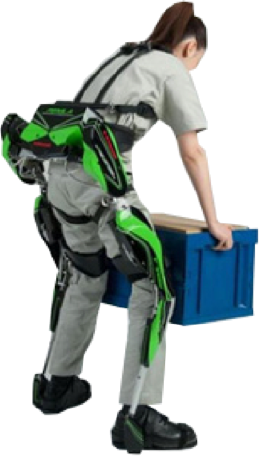
\includegraphics[width=\linewidth]{images/fig_02}

\end{tabular}



\begin{center}
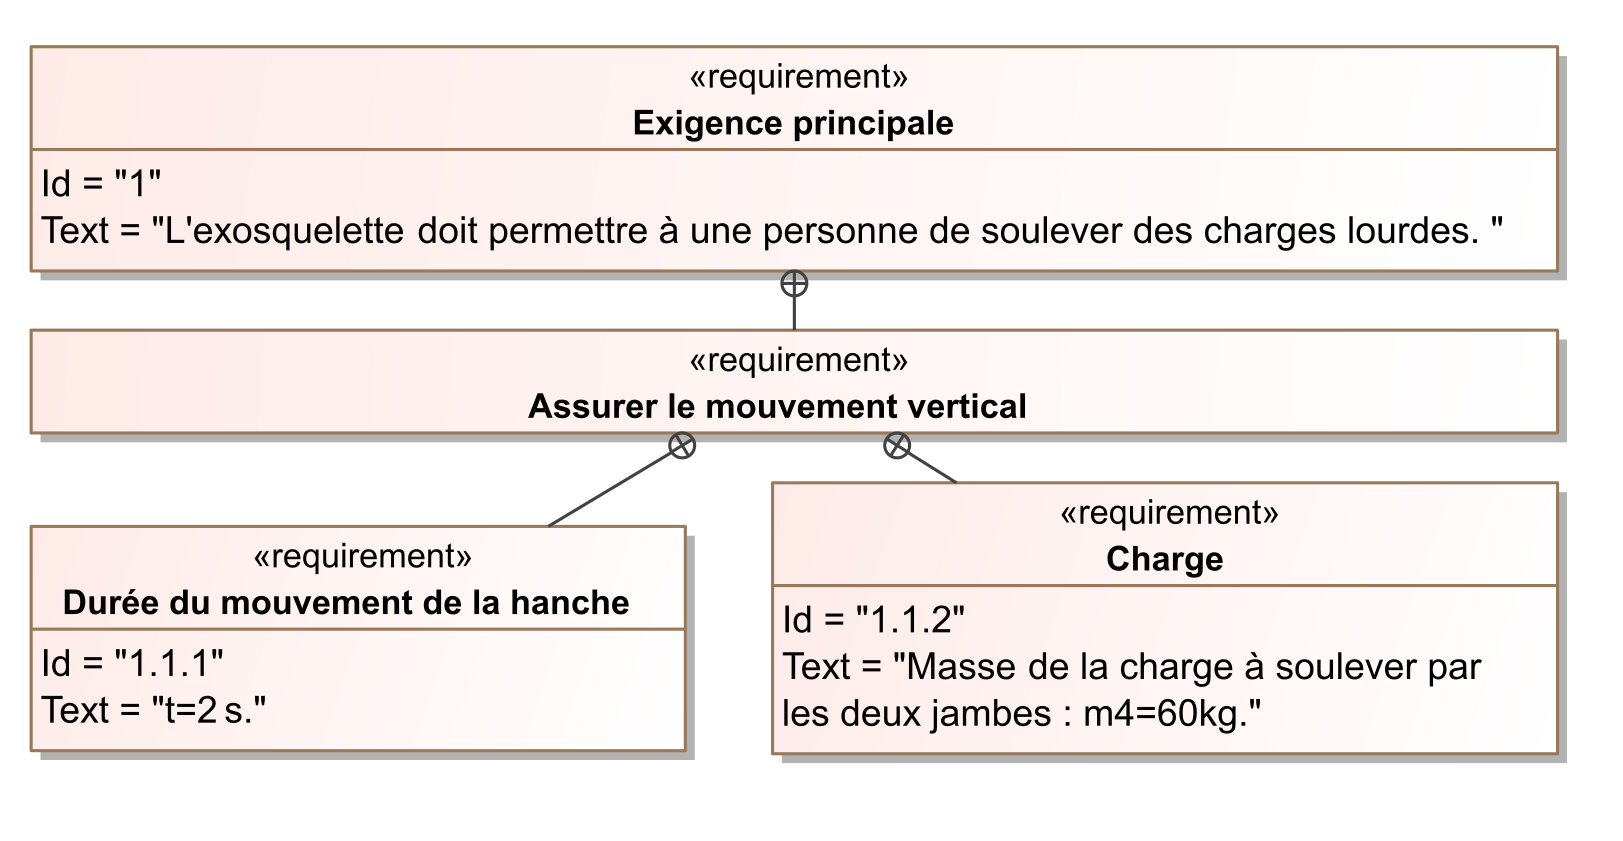
\includegraphics[width=\linewidth]{images/Exigences}
%\textit{}
\end{center}
\fi

%\subsection*{}
\fi
\begin{obj}
Proposer un modèle de connaissance des éléments réalisant l’exigence fonctionnelle <<~assurer le mouvement vertical~>> puis valider les performances attendues listées par le cahier des charges.
\end{obj}



%\subsection*{Élaboration du modèle géométrique direct et du modèle articulaire inverse}
%\begin{obj}
%Élaborer la commande du moteur pilotant le genou à partir d’un mouvement défini dans l’espace
%opérationnel puis converti dans l’espace articulaire.
%\end{obj}
%
%\ifprof
%\else
%L’étude se limite au passage de la position accroupie à la position relevée de l’exosquelette. Lors de ce passage,
%le point $O_2$ est en mouvement de translation verticale suivant la direction $\axe{O_0}{{z_0}}$ et sa vitesse de déplacement
%évolue selon une loi trapézoïdale. Un modèle plan de la chaîne cinématique ouverte représente la partie inférieure
%de l’exosquelette en position debout et fléchie.
%
%
%\begin{center}
%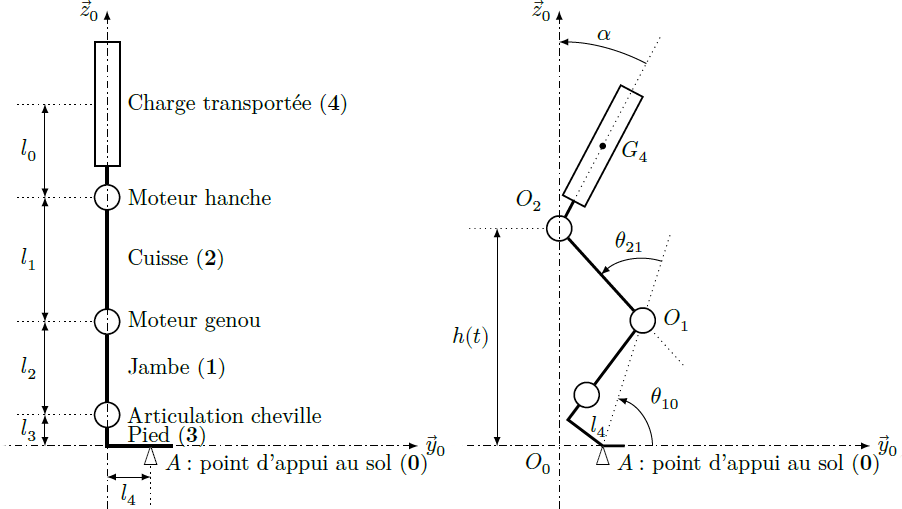
\includegraphics[width=\linewidth]{images/fig_03}
%%\textit{}
%\end{center}
%
%
%%Selon le cahier des charges, pour assurer une bonne synchronisation des axes, l’exigence de précision statique suite à une entrée de type échelon, de type rampe ou de type accélération doit être inférieure à 1\%.
%
%
%On donne le paramétrage du modèle proposé. 
%
%\begin{center}
%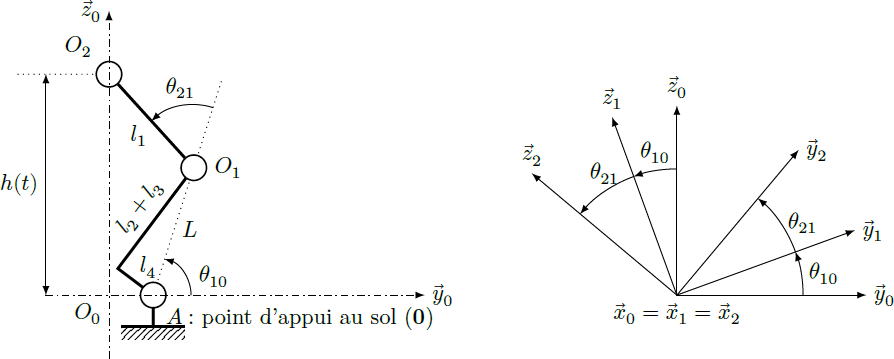
\includegraphics[width=\linewidth]{images/fig_04}
%%\textit{}
%\end{center}
%
%\textbf{Hypothèses : }
%\begin{itemize}
%\item le référentiel lié au repère $\mathcal{R}_0\repere{A}{x_0}{y_0}{z_0}$ est galiléen et est fixe par rapport à la terre;
%\item le point $O_2$ représentant la hanche se déplace verticalement selon la direction $\axe{O_0}{z_0}$;
%\item l’angle $\alpha$ entre la charge transportée et la verticale $\vect{z_0}$ reste constant;
%\item le point d’appui $A$ du pied sur le sol est considéré fixe par rapport à la terre;
%\item lors du mouvement étudié la jambe (1) reste perpendiculaire au pied (3).
%\end{itemize}
%
%\textbf{Données : }
%\begin{itemize}
%\item $\theta_{10}=\angl{y_0}{y_1}=\angl{z_0}{z_1}$;
%\item $\theta_{21}=\angl{y_1}{y_2}=\angl{z_1}{z_2}$;
%\item $\alpha=\text{constante}$;
%\item $L=\sqrt{\left(l_2+l_3\right)^2+l_4^2}$.
%\end{itemize}
%
%\fi
%
%\subparagraph{}\textit{Déterminer littéralement les coordonnées opérationnelles $l_4$ et $h(t)$ en fonction des coordonnées articulaires $\theta_{10}$, $\theta_{21}$ et des paramètres dimensionnels $L$ et $l_1$.}
%\ifprof
%\begin{corrige}
%On a $\vect{A O_1}+\vect{O_1 O_2}+\vect{O_2 O_0}+\vect{O_0 A}=\vect{0}$ soit 
%$L\vect{y_1}+l_1\vect{y_2}-h(t)\vect{z_0}+l_4\vect{y_0}=\vect{0}$. 
%En projetant sur $\vect{y_0}$ et $\vect{z_0}$ on a :
%$$
%\left\{
%\begin{array}{l}
%L\cos\theta_{10} +l_1\cos\left(\theta_{10}+\theta_{21}\right)+l_4={0} \\
%L\sin\theta_{10}  +l_1\sin\left(\theta_{10}+\theta_{21}\right)-h(t) ={0} \\
%\end{array}
%\right.
%$$
%
%En projetant sur $\vect{y_1}$ et $\vect{z_1}$ on a :
%$$
%\left\{
%\begin{array}{l}
%L+l_1\cos\theta_{21}-h(t)\sin\theta_{10}+l_4\cos\theta_{10}={0} \\
%l_1\sin\theta_{21}-h(t)\cos\theta_{10}-l_4\sin\theta_{10}={0}
%\end{array}
%\right.
%$$
%
%
%\end{corrige}
%\else
%\fi
%
%
%\subparagraph{}\textit{Déterminer le modèle articulaire inverse $\theta_{10}$ et $\theta_{21}$ en fonction de $l_1$, $l_4$, $L$ et $h(t)$.}
%\ifprof
%\begin{corrige}
%Pour exprimer $\theta_{10}$, on peut utiliser le premier système d'équation : 
%$$
%\left\{
%\begin{array}{l}
%L\cos\theta_{10}+l_4 =-l_1\cos\left(\theta_{10}+\theta_{21}\right) \\
%L\sin\theta_{10}-h(t)  =-l_1\sin\left(\theta_{10}+\theta_{21}\right) \\
%\end{array}
%\right.
%$$
%En élevant les expressions au carré, on a alors : 
%$
%l_1^2 = \left(L\cos\theta_{10}+l_4 \right)^2+ \left(L\sin\theta_{10}-h(t)\right)^2
%$
%$
%\Leftrightarrow 
%l_1^2 = L^2+l_4^2 +h(t)^2+2Ll_4\cos\theta_{10} -2Lh(t)\sin\theta_{10}
%$
%
%$
%\Leftrightarrow 
%\dfrac{l_1^2 - L^2-l_4^2 -h(t)^2}{2L}=l_4\cos\theta_{10} -h(t)\sin\theta_{10}
%$
%
%En utilisant l'indication, on a : 
%$$
%\dfrac{l_4}{\sqrt{l_4^2 + h(t)^2}}\cos\theta_{10} +\dfrac{-h(t)}{\sqrt{l_4^2 + h(t)^2}}\sin\theta_{10}=\dfrac{l_1^2 - L^2-l_4^2 -h(t)^2}{2L{\sqrt{l_4^2 + h(t)^2}}}
%$$
%En conséquence, on pose $\cos\varphi=\dfrac{l_4}{\sqrt{l_4^2 + h(t)^2}}$ et 
%$\sin\varphi = \dfrac{-h(t)}{\sqrt{l_4^2 + h(t)^2}}$. 
%En conséquences %$\tan\varphi = \dfrac{\dfrac{-h(t)}{\sqrt{l_4^2 + h(t)^2}}}{\dfrac{l_4}{\sqrt{l_4^2 + h(t)^2}}}=\dfrac{-h(t)}{l_4}$.
%$\tan\varphi =\dfrac{-h(t)}{l_4}$.
%
%
%Par suite, $\cos\left( \theta_{10} - \varphi \right) =\dfrac{l_1^2 - L^2-l_4^2 -h(t)^2}{2L{\sqrt{l_4^2 + h(t)^2}}}$. On a donc 
%$\theta_{10} =\arccos \left( \dfrac{l_1^2 - L^2-l_4^2 -h(t)^2}{2L{\sqrt{l_4^2 + h(t)^2}}}\right) + \varphi$.
%
%
%Au final, 
%$$\theta_{10} =\arccos \left( \dfrac{l_1^2 - L^2-l_4^2 -h(t)^2}{2L{\sqrt{l_4^2 + h(t)^2}}}\right) + \arctan\left(\dfrac{-h(t)}{l_4} \right).$$
%
%Pour exprimer  $\theta_{21}$ on réutilise le premier système d'équations :
%$
%\left\{
%\begin{array}{l}
%-l_4 =l_1\cos\left(\theta_{10}+\theta_{21}\right) + L\cos\theta_{10} \\
%h(t)  =l_1\sin\left(\theta_{10}+\theta_{21}\right) + L\sin\theta_{10}\\
%\end{array}
%\right.
%$
%
%On a alors 
%$l_4 ^2 +h(t)^2= L^2 + l_1^2 + 2l_1L\left(\cos\theta_{10}\cos\left(\theta_{10}+\theta_{21}\right) +\sin\left(\theta_{10}+\theta_{21}\right) \sin\theta_{10}\right)$.
%En conséquences, 
%$\dfrac{l_4 ^2 +h(t)^2- L^2 - l_1^2}{2l_1L} = \cos\theta_{10}\cos\left(\theta_{10}+\theta_{21}\right) +\sin\left(\theta_{10}+\theta_{21}\right) \sin\theta_{10}$
%$= \cos\left(\theta_{10}+\theta_{21}-\theta_{10}\right) $.
%D'où $\theta_{21}=\arccos\left(\dfrac{l_4 ^2 +h(t)^2- L^2 - l_1^2}{2l_1L}  \right)$.
%\end{corrige}
%
%
%\else
%\fi
%
%\ifprof
%\else
%\begin{methode}
%Lorsqu'on a une équation de la forme $A\cos\theta_{10}+B\sin\theta_{10}=C$. On peut normer cette équation en la mettant sous la forme $\dfrac{A}{\sqrt{A^2+B^2}}\cos\theta_{10}+\dfrac{B}{\sqrt{A^2+B^2}}\sin\theta_{10}=\dfrac{C}{\sqrt{A^2+B^2}}$.
%On pose alors $\cos\varphi = \dfrac{A}{\sqrt{A^2+B^2}}$ et $\sin\varphi=\dfrac{B}{\sqrt{A^2+B^2}}$. On a alors $\cos\left( \theta_{10} - \varphi \right)=\dfrac{C}{\sqrt{A^2+B^2}}$.
%\end{methode}
%\fi
%
%\subsection*{Élaboration du modèle cinématique}
%\begin{obj}
%En vue de dimensionner le moteur du genou, déterminer la vitesse articulaire en fonction de la  vitesse opérationnelle.
%\end{obj}
%
%\subparagraph{}\textit{Déterminer à partir du modèle articulaire inverse la vitesse angulaire 
%$\theta_{21}$ en fonction de $h(t)$, $\dot{h}(t)$, $l_1$, $L$ et $\sin\theta_{21}$.}
%\ifprof
%\begin{corrige}
%On a vu que $\cos\theta_{21}=\dfrac{l_4 ^2 +h(t)^2- L^2 - l_1^2}{2l_1L}  $.
%En dérivant, on a donc $- \dot{\theta}_{21} \sin\theta_{21}=\dfrac{2\dot{h}(t)h(t)}{2l_1L}$.
%Au final,  $\dot{\theta}_{21} =-\dfrac{\dot{h}(t)h(t)}{l_1L\sin\theta_{21}}$.
%\end{corrige}
%\else
%\fi
%
%\ifprof
%\else
%Un modèle multiphysique a permis de déterminer les conditions suivantes correspondant à la vitesse maximale : $t=\SI{1,5}{s}$, $h(t=1,5)=\SI{0,829}{m}$, $\dot{h}(t=1,5)=\SI{0,422}{m.s^{-1}}$ et $\theta_{21} = 55,9\degres$. Les longueurs $l_1$ et $L$ valent
%respectivement \SI{43,1}{cm} et \SI{51,8}{cm}. Le réducteur de vitesse utilisé a un rapport de réduction égal à $r=\dfrac{1}{120}$.
%\fi
%
%\subparagraph{}\textit{Déterminer la valeur maximale de la vitesse angulaire $\dot{\theta}_{21}$ et $\text{rad s}^{-1}$ puis celle de la fréquence de rotation d’un moteur de genou en $\text{tr min}^{-1}$.}
%\ifprof
%\begin{corrige}
%On a : $\dot{\theta}_{21} =-\dfrac{0,422 \times 0,829}{0,431\times 0,518\sin \left(55,9\right)}\simeq -\SI{1,89}{rad.s^{-1}}$. Soit une fréquence de rotation du moteur de \SI{2168}{tr.min^{-1}}.
%\end{corrige}
%\else
%\fi


\subsection*{Élaboration du modèle dynamique}

\begin{obj}
Dimensionner le moteur situé au niveau d’un genou permettant à l’exosquelette de soulever une masse de \SI{60}{kg} de la position accroupie à la position debout.
\end{obj}

Ces calculs visent à déterminer l’équation dynamique qui permet d’obtenir le couple moteur (minimal) en fonction des caractéristiques géométriques et massique de la charge à soulever ainsi que des conditions d’utilisation.
Le modèle d’étude est celui représenté à la figure suivante correspondant au modèle d’étude plan position fléchie.
\begin{center}
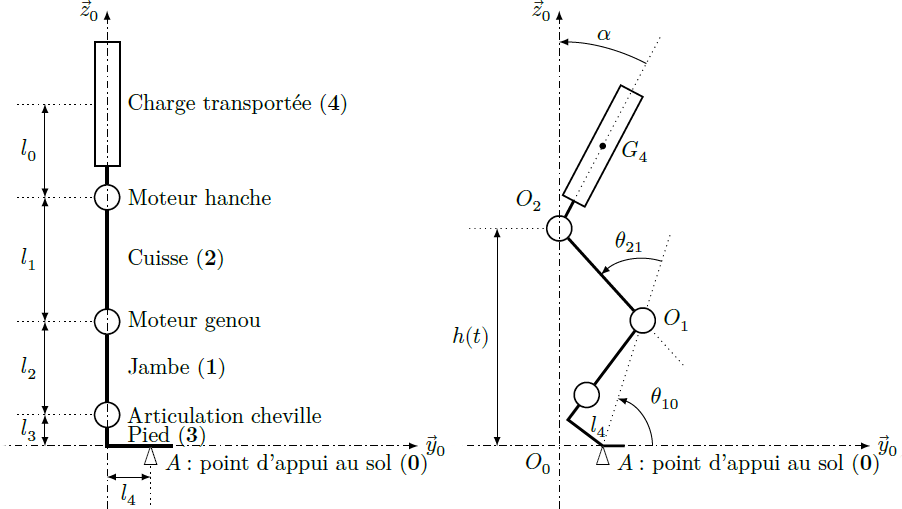
\includegraphics[width=\linewidth]{images/fig_03}
%\textit{}
\end{center}

\begin{center}
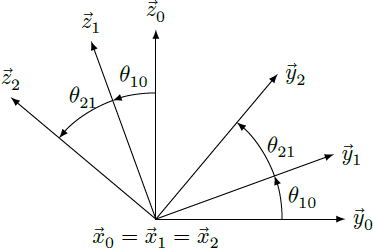
\includegraphics[width=.7\linewidth]{images/fig_14}
%\textit{}
\end{center}


\noindent\textbf{Hypothèses :}
\begin{itemize}
\item L’étude est modélisable dans le plan.
\item Toutes les liaisons sont supposées parfaites.
\item Les inerties des pièces sont négligées sauf la masse de la charge à soulever.
\item L’angle $\alpha$ entre la charge transportée et la verticale$\vect{z_0}$ reste constant.
\item $G_4$, centre de gravité de la charge transportée (4), reste en permanence à la verticale du point $A$ d’appui au sol.
\end{itemize}

\noindent\textbf{Données :}
\begin{itemize}
\item $\vect{O_1G_4}=\lambda(t)\vect{z_0}-L\cos\theta_{10}\vect{y_0}$;
\item Accélération de la pesanteur $g=\SI{9,81}{m.s^{-2}}$;
\item Longueur de la cuisse $l_1 = \SI{43,1}{cm}$.
\item Longueur de la jambe $l_2 = \SI{43,3}{cm}$.
\item Longueur de l'articulation de la cheville à la plante arrière du pied $l_3 = \SI{6,9}{cm}$.
\item Longueur de la plante arrière du pied au point d’appui sur le sol $l_4 = \SI{13}{cm}$.
\item Longueur $\vect{O_0O_1}=L\vect{y_1}$ avec $L=\SI{51,8}{cm}$.
\item Rapport de réduction : $r=\dfrac{1}{120}$.
\end{itemize}

On note E=\{cuisse(2)+charge transportée(4)\}. 

\subparagraph{} \textit{Donner qualitativement le mouvement de 4 par rapport à 0. Tracer le graphe de structure du système.}

\ifprof
\begin{corrige}
Étant donné que l'on souhaite que l'angle $\alpha$ reste constant pendant la levée d'une charge, le mouvement de $E$ sera donc un mouvement de translation rectiligne.  
\end{corrige}
\else
\fi


\subparagraph{} \textit{Déterminer $\vectmc{O_1}{E}{0}\cdot \vect{x_0}$ en fonction de $m_4$, $\dot{h}(t)$, $L$ et $\cos\theta_{10}$.}

\ifprof
\begin{corrige}
$E$ étant en translation, on a $\vectmc{G_4}{E}{0}=\vect{0}$. On a alors 
 $\vectmc{O_1}{E}{0}=\vectmc{G_4}{E}{0}+\vect{O_1G_4}\wedge\vectrc{E}{0}$.

Par ailleurs, $\vectrc{E}{0}=m_4\vectv{G_4}{E}{0} = m_4\dot{h}(t)\vect{z_0}$. 

On a donc :
$ \vectmc{O_1}{E}{0}\cdot \vect{x_0} 
= \left(\left( \lambda(t)\vect{z_0}-L\cos\theta_{10}\vect{y_0}\right)\wedge m_4\dot{h}(t)\vect{z_0}\right) \cdot \vect{x_0}
=  -Lm_4\cos\theta_{10}\dot{h}(t)$.
 
 
\end{corrige}
\else
\fi



\subparagraph{} \textit{Déduire $\vectmd{O_1}{E}{0}\cdot \vect{x_0}$ en fonction de $m_4$, $\ddot{h}(t)$, $L$ et $\cos\theta_{10}$.}

\ifprof
\begin{corrige}
\subsubsection*{Méthode 1 -- Calcul de $\vectmd{G_4}{E}{0}$ et déplacement}
On a $\vectmd{G_4}{E}{0}= \dfrac{\dd \vectmc{G_4}{E}{0}}{\dd t}= \vect{0}$. En conséquences, 
$ \vectmd{O_1}{E}{0}\cdot \vect{x_0} 
= \left(\left( \lambda(t)\vect{z_0}-L\cos\theta_{10}\vect{y_0}\right)\wedge m_4\ddot{h}(t)\vect{z_0}\right) \cdot \vect{x_0} =  -Lm_4\cos\theta_{10}\ddot{h}(t)$.

\subsubsection*{Méthode 2 -- Calcul de $\vectmd{O_1}{E}{0}$}
On a aussi $\vectmd{O_1}{E}{0} = \left(\dfrac{d \vectmc{O_1}{E}{0}}{\dd t}\right)+m_4\vect{V\left(O_1/0\right)}\wedge\vectv{G_4}{E}{0} $. 

Par suite on a 
$\left(\vectv{O_1}{E}{0}\wedge\vectv{G_4}{E}{0}\right)\vect{x_0}=
\left(\left( L\vect{y_1}\wedge \dot{\theta}_{10} \vect{x_0} \right) \wedge\dot{h}(t)\vect{z_0}\right)\vect{x_0} 
= \left( -L\dot{\theta}_{10} \vect{z_1} \wedge\dot{h}(t)\vect{z_0}\right)\vect{x_0} $ 
$= -L\dot{\theta}_{10} \dot{h}(t) \sin \theta_{10} $. 

Enfin, 
 $\vectmd{O_1}{E}{0}\cdot\vect{x_0}=-Lm_4\cos\theta_{10}\ddot{h}(t)+Lm_4\dot{\theta}_{10}\sin\theta_{10}\dot{h}(t)-m_4L\dot{\theta}_{10} \dot{h}(t) \sin \theta_{10}$
 $=-Lm_4\cos\theta_{10}\ddot{h}(t)$.


 
\end{corrige}
\else
\fi

La loi d'évolution de la vitesse de la hanche est donnée à la figure suivante. 

\begin{center}
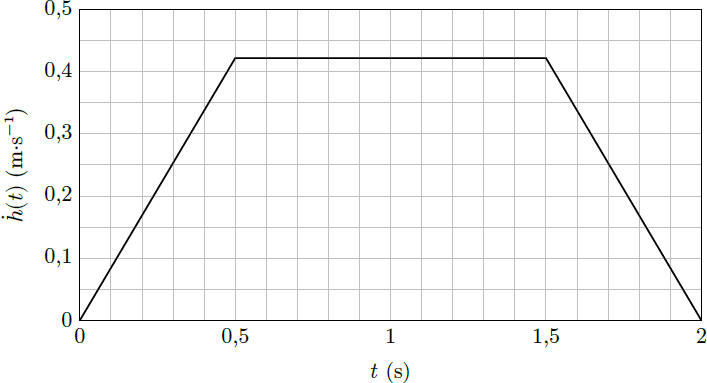
\includegraphics[width=\linewidth]{images/fig_11}
%\textit{}
\end{center}


\subparagraph{} \textit{Déterminer l’expression littérale du couple $C_r$ exercé par l’arbre de sortie du réducteur sur le genou imposé par la loi d’évolution de la hanche et calculer numériquement ce couple pour une valeur de $\theta_{10}$ égale à
54,5\degres correspondant à la valeur maximale du couple.}

\ifprof
\begin{corrige}
\begin{itemize}
\item On isole l'ensemble $E$.
\item On réalise le bilan des actions mécaniques : 
\begin{itemize}
\item action de la liaison pivot : $\torseurstat{T}{1}{E}=\torseurl{\vectf{1}{E}}{\vectm{O_1}{1}{E}}{O_1}$ avec $\vectm{O_1}{1}{E}\cdot \vect{x_0}=0$;
\item action du réducteur: $\torseurstat{T}{1_r}{E}=\torseurl{\vect{0}}{C_r \vect{x_0}}{O_1}$ avec $\vectm{O_1}{1}{E}\cdot \vect{x_0}=0$;
\item action de la pesanteur : 
$\torseurstat{T}{\text{pes}}{E}=\torseurl{-m_4g\vect{z_0}}{\vect{0}}{G_4}$. On a alors 
$\vectm{O_1}{\text{pes}}{E}\cdot \vect{x_0}=\vectm{G_4}{\text{pes}}{E}\cdot \vect{x_0}+\left(\vect{O_1G_4}\wedge -m_4g\vect{z_0} \right)\cdot \vect{x_0}$  
$=\left(\left(\lambda(t)\vect{z_0}-L\cos\theta_{10}\vect{y_0}\right)\wedge -m_4g\vect{z_0} \right)\cdot \vect{x_0}$ 
$=\left(-L\cos\theta_{10}\vect{y_0}\wedge -m_4g\vect{z_0}\right)\cdot \vect{x_0}$ $= m_4gL\cos\theta_{10}$.
\end{itemize}
\item $E$ étant en pivot d'axe $\axe{O_1}{{x_1}}$, on applique le théorème du moment dynamique en $O_1$ en projection sur $\vect{x_1}$ :
$-Lm_4\cos\theta_{10}\ddot{h}(t) =C_r +m_4gL\cos\theta_{10}$
$ \Leftrightarrow C_r=-m_4 L \cos\theta_{10} \left(g+\ddot{h}(t)\right) $. 
\end{itemize}

En réalisant l'application numérique, on a : $C_r = - 60 \times 51,8\times 10^{-2}\times \cos 54,5 \left(9,81 +\dfrac{0,425}{0,5} \right)  $


\end{corrige}

\else
\fi



\subparagraph{} \textit{Calculer le couple $C_m$ au niveau de l’arbre moteur du genou en prenant un facteur de perte $\eta = 0,75$ (estimé à l’aide du modèle multiphysique).}
\ifprof
\begin{corrige}
En régime permanent, on a $\eta=\dfrac{C_r \omega_r}{C_m \omega_m}=r\dfrac{C_r}{C_m}$ et $C_r = \dfrac{\eta}{r}C_m$=.
\end{corrige}
\else
\fi



\subparagraph{} \textit{Expliquer en moins de 5 lignes comment estimer un rendement à partir d'un modèle multiphysique.}
\ifprof
\begin{corrige}
\end{corrige}
\else
\fi

\subsection*{Validation du dimensionnement du moteur}
\begin{obj}
Vérifier que le moteur choisi convient pour une utilisation intensive comprenant 4 cycles par minute
de descente suivie d’une montée.
\end{obj}

Le cycle suivant obtenu à l’aide du modèle multiphysique de représente l’évolution du couple moteur,
et ce en tenant compte du moment d’inertie du rotor, sur un cycle de période $T=\SI{15}{s}$.


\noindent Quatre phases sont définies sur cette période :
\begin{itemize}
\item phase 1 pour $0 \leq t < \SI{2}{s}$, valeur efficace du couple moteur $C_1 = \SI{0,838}{Nm}$ ;
\item phase 2 pour $2 \leq t < \SI{4}{s}$, couple moteur constant $C_2 = -\SI{0,912}{Nm}$ ;
\item phase 3 pour $4 \leq t < \SI{6}{s}$, valeur efficace du couple moteur $C_3 = \SI{0,838}{Nm}$;
\item phase 4 pour $6 \leq t < \SI{15}{s}$, couple moteur nul.
\end{itemize}



\begin{center}
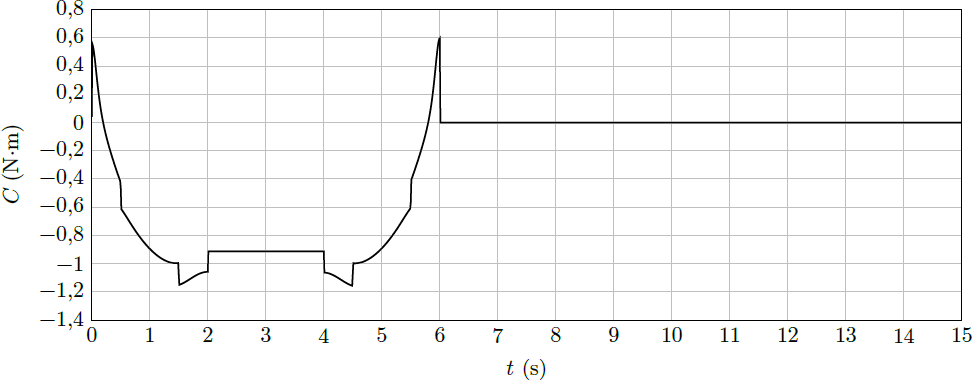
\includegraphics[width=\linewidth]{images/fig_12}
%\textit{}
\end{center}


\subparagraph{} \textit{Préciser à quels mouvements correspondent les 4 phases de ce cycle.}

\ifprof
\begin{corrige}
\begin{itemize}
\item Phase 1 : le couple est décroissant, suivant la convention de signe utilisée, on peut faire l'hypothèse que le genou fléchit et que l’accélération est décroissante.
\item Phase 2 : le couple est constant. On peut faire l'hypothèse que le moteur tourne à vitesse constante et que le couple moteur est celui nécessaire à vaincre les frottements. 
\item Phase 3 : le couple est croissant. En conservant la même << convention >> que précédemment, le genou ralentit et arrive en fin de flexion .
\item Phase 4 : si le genou ne bouge plus, on peut faire l'hypothèse que l'exosquelette est en butée. Ainsi, il n'est pas nécessaire d'avoir un couple pour maintenir le système en position.
\end{itemize}
\end{corrige}
\else
\fi

Le couple efficace est également appelé couple thermiquement équivalent, il est défini par :
$C_{\text{eff}}=\sqrt{\dfrac{1}{T}\int\limits_0^Tc(t)^2 \dd t}$. On a aussi 
$C_{\text{eff}}=\sqrt{\dfrac{1}{T}\sum\limits_{i=1}^n C_{\text{i,eff}}^2 T_i }$


\subparagraph{} \textit{Calculer la valeur efficace du couple moteur du genou pour ce cycle périodique de \SI{15}{s}.}

\ifprof
\begin{corrige}
$C_{\text{eff}}=\sqrt{\dfrac{1}{T}\sum\limits_{i=1}^n C_{\text{i,eff}}^2 T_i }$
$=\sqrt{\dfrac{1}{15}\left(0,838^2 \times 2 +0,912^2 \times 2 + 0,838^2 \times 2 \right) }\simeq \SI{0,546}{Nm}$.
\end{corrige}
\else
\fi
Le couple moteur varie entre \SI{-1,156}{Nm} et \SI{0,596}{Nm}.
Les caractéristiques du moteur choisi sont :
\begin{itemize}
\item vitesse à vide de \SI{3120}{tr.min^{-1}} pour une alimentation nominale en amont de l’onduleur de \SI{36}{V};
\item couple permanent admissible de \SI{0,560}{Nm};
\item pente de la courbe de la vitesse en fonction du couple de \SI{423}{tr.min^{-1}N^{-1}m^{-1}}.
\end{itemize}

De plus une étude cinématique précédente a montré que le moteur permettant d'actionner le moteur doit pouvoir atteindre une vitesse de \SI{2200}{tr.min^{-1}}.


\subparagraph{} \textit{Conclure quant au choix de ce moteur au regard de la valeur maximale de la vitesse angulaire calculée lors d'une étude précédente et du couple efficace calculé à la question précédente.}

\ifprof
\begin{corrige}
\begin{enumerate}
\item Le couple thermiquement équivalent calculé est de \SI{0,546}{Nm} ce qui est inférieur aux couple admissible par le moteur. 
\item La fréquence de rotation à atteindre par le moteur est de \SI{2200}{tr.min^{-1}}. Le moteur proposé tourne à \SI{3120}{tr.min^{-1}} à vide. On peut donc supposer qu'en charge, il atteindre les \SI{2200}{tr.min^{-1}}.
\end{enumerate}
Su ces deux critères le moteur proposé est donc validé. 
\end{corrige}
\else
\fi

\ifprof
\else

\noindent 
\footnotesize
\begin{tabular}{|p{.95\linewidth}|}
\hline
Éléments de corrigé :
\begin{enumerate}
\item ....
\end{enumerate} \\
\hline
\end{tabular}
\normalsize
\fi

\ifprof
\else
\end{multicols}
\fi



\begin{center}
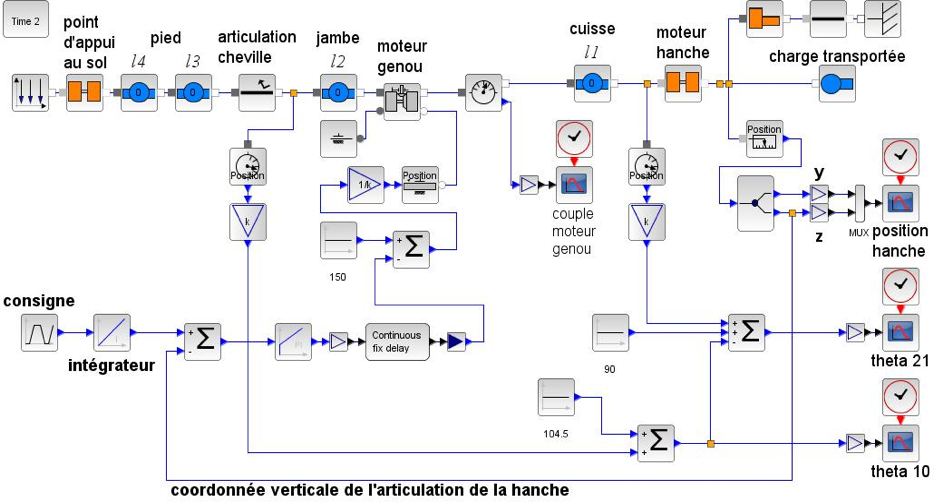
\includegraphics[width=\linewidth]{images/fig_07}
%\textit{}
\end{center}

%\begin{center}
%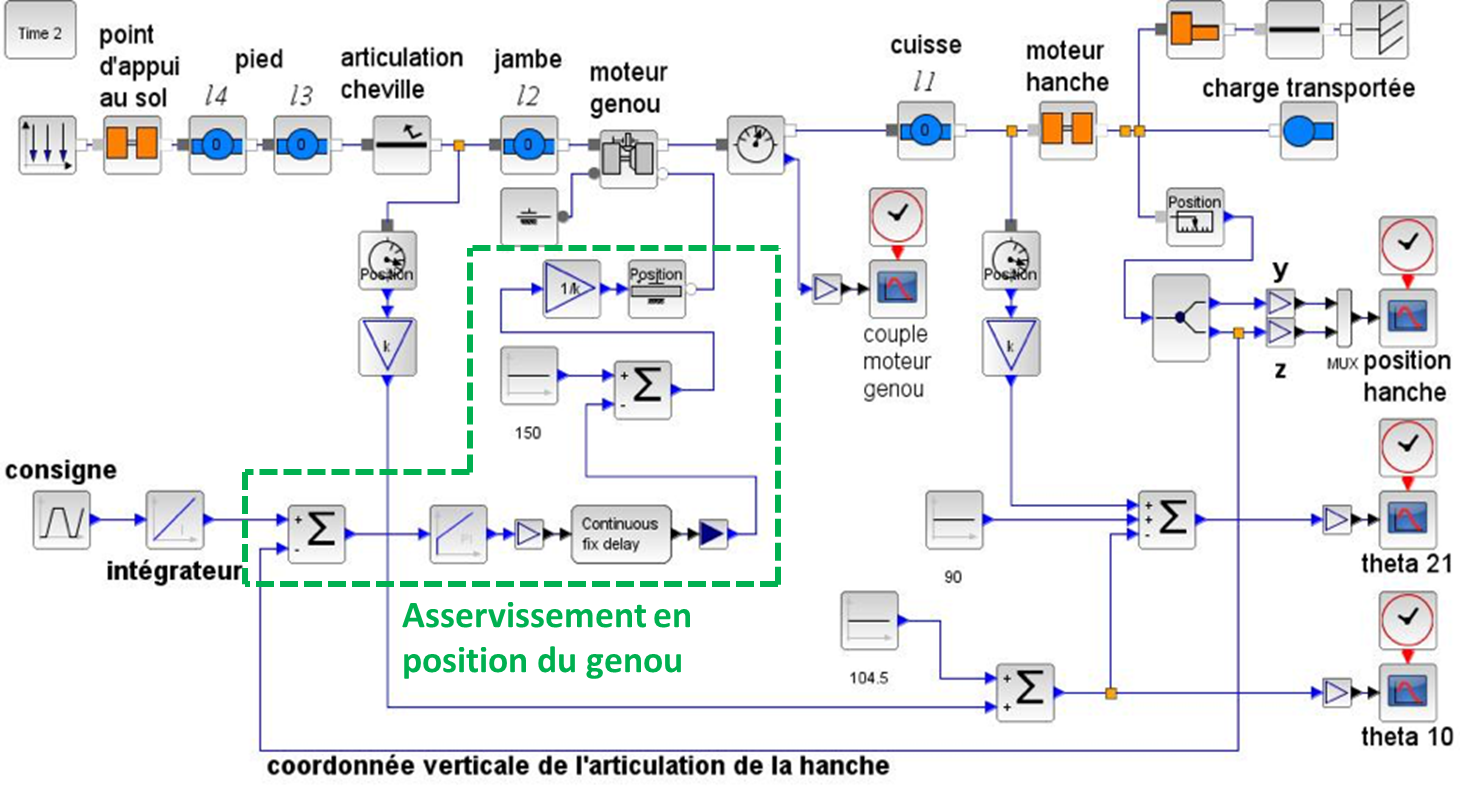
\includegraphics[width=.65\linewidth]{images/cor_01}
%%\textit{}
%\end{center}

\end{document}
